The \texttt{\pkglnk{model.parsing}} package contains the classes necessary to turn an input String into a lambda term object.
This process is initiate by the \texttt{\lnk{ExecutionEngine}} instancing a new \texttt{\lnk{Parser}} object with the currently activated libraries and invoking its parse method. The Parser in turn uses the \texttt{\lnk{Tokeniser}} to turn the input String into a sequence of Tokens. 

Each \texttt{\lnk{Token}} contains a section of original input String. This substring is passed to the Token on its creation by the Tokeniser and can be access trough the Token's interface.

From this sequence the Parser builds a lambda term object structure.
If the input contains names referencing library terms and the Parser is initialized with the necessary libraries, the terms will be incorporated in the lambda term object and their names conserved.
 
If the input String can not be parsed a \texttt{\lnk{ParseEception}} is thrown.
The \texttt{\lnk{ParseEception}} contains an error message describing the error which led to its creation, and where in the input String the error occurred.
Both message and location can accessed and printed to the output window to aid the user in correcting the error.

\begin{figure}[H]
	\centering
	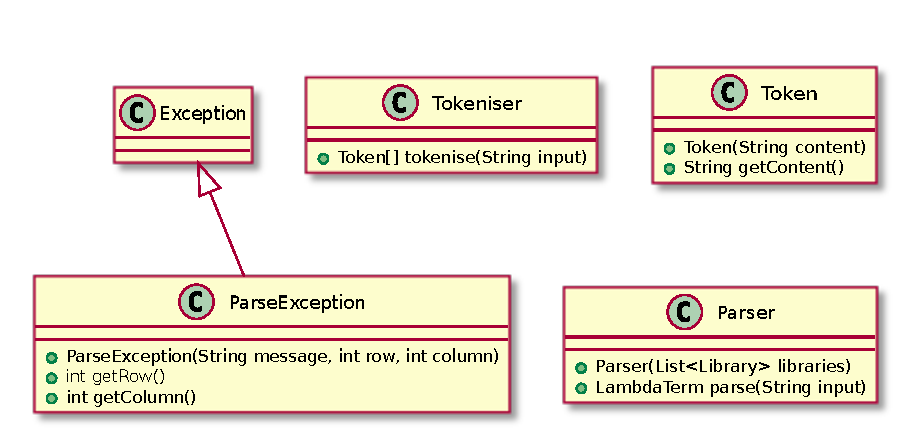
\includegraphics[width=\textwidth]{packageDiagrams/parsingPackage}
\end{figure}
